\documentclass[1p]{elsarticle_modified}
%\bibliographystyle{elsarticle-num}

%\usepackage[colorlinks]{hyperref}
%\usepackage{abbrmath_seonhwa} %\Abb, \Ascr, \Acal ,\Abf, \Afrak
\usepackage{amsfonts}
\usepackage{amssymb}
\usepackage{amsmath}
\usepackage{amsthm}
\usepackage{scalefnt}
\usepackage{amsbsy}
\usepackage{kotex}
\usepackage{caption}
\usepackage{subfig}
\usepackage{color}
\usepackage{graphicx}
\usepackage{xcolor} %% white, black, red, green, blue, cyan, magenta, yellow
\usepackage{float}
\usepackage{setspace}
\usepackage{hyperref}

\usepackage{tikz}
\usetikzlibrary{arrows}

\usepackage{multirow}
\usepackage{array} % fixed length table
\usepackage{hhline}

%%%%%%%%%%%%%%%%%%%%%
\makeatletter
\renewcommand*\env@matrix[1][\arraystretch]{%
	\edef\arraystretch{#1}%
	\hskip -\arraycolsep
	\let\@ifnextchar\new@ifnextchar
	\array{*\c@MaxMatrixCols c}}
\makeatother %https://tex.stackexchange.com/questions/14071/how-can-i-increase-the-line-spacing-in-a-matrix
%%%%%%%%%%%%%%%

\usepackage[normalem]{ulem}

\newcommand{\msout}[1]{\ifmmode\text{\sout{\ensuremath{#1}}}\else\sout{#1}\fi}
%SOURCE: \msout is \stkout macro in https://tex.stackexchange.com/questions/20609/strikeout-in-math-mode

\newcommand{\cancel}[1]{
	\ifmmode
	{\color{red}\msout{#1}}
	\else
	{\color{red}\sout{#1}}
	\fi
}

\newcommand{\add}[1]{
	{\color{blue}\uwave{#1}}
}

\newcommand{\replace}[2]{
	\ifmmode
	{\color{red}\msout{#1}}{\color{blue}\uwave{#2}}
	\else
	{\color{red}\sout{#1}}{\color{blue}\uwave{#2}}
	\fi
}

\newcommand{\Sol}{\mathcal{S}} %segment
\newcommand{\D}{D} %diagram
\newcommand{\A}{\mathcal{A}} %arc


%%%%%%%%%%%%%%%%%%%%%%%%%%%%%5 test

\def\sl{\operatorname{\textup{SL}}(2,\Cbb)}
\def\psl{\operatorname{\textup{PSL}}(2,\Cbb)}
\def\quan{\mkern 1mu \triangleright \mkern 1mu}

\theoremstyle{definition}
\newtheorem{thm}{Theorem}[section]
\newtheorem{prop}[thm]{Proposition}
\newtheorem{lem}[thm]{Lemma}
\newtheorem{ques}[thm]{Question}
\newtheorem{cor}[thm]{Corollary}
\newtheorem{defn}[thm]{Definition}
\newtheorem{exam}[thm]{Example}
\newtheorem{rmk}[thm]{Remark}
\newtheorem{alg}[thm]{Algorithm}

\newcommand{\I}{\sqrt{-1}}
\begin{document}

%\begin{frontmatter}
%
%\title{Boundary parabolic representations of knots up to 8 crossings}
%
%%% Group authors per affiliation:
%\author{Yunhi Cho} 
%\address{Department of Mathematics, University of Seoul, Seoul, Korea}
%\ead{yhcho@uos.ac.kr}
%
%
%\author{Seonhwa Kim} %\fnref{s_kim}}
%\address{Center for Geometry and Physics, Institute for Basic Science, Pohang, 37673, Korea}
%\ead{ryeona17@ibs.re.kr}
%
%\author{Hyuk Kim}
%\address{Department of Mathematical Sciences, Seoul National University, Seoul 08826, Korea}
%\ead{hyukkim@snu.ac.kr}
%
%\author{Seokbeom Yoon}
%\address{Department of Mathematical Sciences, Seoul National University, Seoul, 08826,  Korea}
%\ead{sbyoon15@snu.ac.kr}
%
%\begin{abstract}
%We find all boundary parabolic representation of knots up to 8 crossings.
%
%\end{abstract}
%\begin{keyword}
%    \MSC[2010] 57M25 
%\end{keyword}
%
%\end{frontmatter}

%\linenumbers
%\tableofcontents
%
\newcommand\colored[1]{\textcolor{white}{\rule[-0.35ex]{0.8em}{1.4ex}}\kern-0.8em\color{red} #1}%
%\newcommand\colored[1]{\textcolor{white}{ #1}\kern-2.17ex	\textcolor{white}{ #1}\kern-1.81ex	\textcolor{white}{ #1}\kern-2.15ex\color{red}#1	}

{\Large $\underline{12n_{0114}~(K12n_{0114})}$}

\setlength{\tabcolsep}{10pt}
\renewcommand{\arraystretch}{1.6}
\vspace{1cm}\begin{tabular}{m{100pt}>{\centering\arraybackslash}m{274pt}}
\multirow{5}{120pt}{
	\centering
	\includegraphics[width=112pt]{../../../GIT/diagram.site/Diagrams/png/2203_12n_0114.png}\\
\ \ \ A knot diagram\footnotemark}&
\allowdisplaybreaks
\textbf{Linearized knot diagam} \\
\cline{2-2}
 &
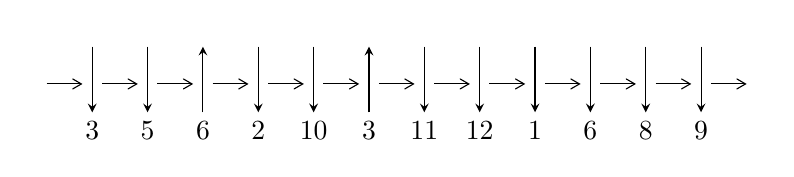
\begin{tikzpicture}[x=20pt, y=17pt]
	% nodes
	\node (C0) at (0, 0) {};
	\node (C1) at (1, 0) {};
	\node (C1U) at (1, +1) {};
	\node (C1D) at (1, -1) {3};

	\node (C2) at (2, 0) {};
	\node (C2U) at (2, +1) {};
	\node (C2D) at (2, -1) {5};

	\node (C3) at (3, 0) {};
	\node (C3U) at (3, +1) {};
	\node (C3D) at (3, -1) {6};

	\node (C4) at (4, 0) {};
	\node (C4U) at (4, +1) {};
	\node (C4D) at (4, -1) {2};

	\node (C5) at (5, 0) {};
	\node (C5U) at (5, +1) {};
	\node (C5D) at (5, -1) {10};

	\node (C6) at (6, 0) {};
	\node (C6U) at (6, +1) {};
	\node (C6D) at (6, -1) {3};

	\node (C7) at (7, 0) {};
	\node (C7U) at (7, +1) {};
	\node (C7D) at (7, -1) {11};

	\node (C8) at (8, 0) {};
	\node (C8U) at (8, +1) {};
	\node (C8D) at (8, -1) {12};

	\node (C9) at (9, 0) {};
	\node (C9U) at (9, +1) {};
	\node (C9D) at (9, -1) {1};

	\node (C10) at (10, 0) {};
	\node (C10U) at (10, +1) {};
	\node (C10D) at (10, -1) {6};

	\node (C11) at (11, 0) {};
	\node (C11U) at (11, +1) {};
	\node (C11D) at (11, -1) {8};

	\node (C12) at (12, 0) {};
	\node (C12U) at (12, +1) {};
	\node (C12D) at (12, -1) {9};
	\node (C13) at (13, 0) {};

	% arrows
	\draw[->,>={angle 60}]
	(C0) edge (C1) (C1) edge (C2) (C2) edge (C3) (C3) edge (C4) (C4) edge (C5) (C5) edge (C6) (C6) edge (C7) (C7) edge (C8) (C8) edge (C9) (C9) edge (C10) (C10) edge (C11) (C11) edge (C12) (C12) edge (C13) ;	\draw[->,>=stealth]
	(C1U) edge (C1D) (C2U) edge (C2D) (C3D) edge (C3U) (C4U) edge (C4D) (C5U) edge (C5D) (C6D) edge (C6U) (C7U) edge (C7D) (C8U) edge (C8D) (C9U) edge (C9D) (C10U) edge (C10D) (C11U) edge (C11D) (C12U) edge (C12D) ;
	\end{tikzpicture} \\
\hhline{~~} \\& 
\textbf{Solving Sequence} \\ \cline{2-2} 
 &
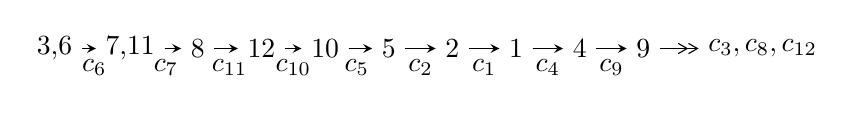
\begin{tikzpicture}[x=23pt, y=7pt]
	% node
	\node (A0) at (-1/8, 0) {3,6};
	\node (A1) at (17/16, 0) {7,11};
	\node (A2) at (17/8, 0) {8};
	\node (A3) at (25/8, 0) {12};
	\node (A4) at (33/8, 0) {10};
	\node (A5) at (41/8, 0) {5};
	\node (A6) at (49/8, 0) {2};
	\node (A7) at (57/8, 0) {1};
	\node (A8) at (65/8, 0) {4};
	\node (A9) at (73/8, 0) {9};
	\node (C1) at (1/2, -1) {$c_{6}$};
	\node (C2) at (13/8, -1) {$c_{7}$};
	\node (C3) at (21/8, -1) {$c_{11}$};
	\node (C4) at (29/8, -1) {$c_{10}$};
	\node (C5) at (37/8, -1) {$c_{5}$};
	\node (C6) at (45/8, -1) {$c_{2}$};
	\node (C7) at (53/8, -1) {$c_{1}$};
	\node (C8) at (61/8, -1) {$c_{4}$};
	\node (C9) at (69/8, -1) {$c_{9}$};
	\node (A10) at (11, 0) {$c_{3},c_{8},c_{12}$};

	% edge
	\draw[->,>=stealth]	
	(A0) edge (A1) (A1) edge (A2) (A2) edge (A3) (A3) edge (A4) (A4) edge (A5) (A5) edge (A6) (A6) edge (A7) (A7) edge (A8) (A8) edge (A9) ;
	\draw[->>,>={angle 60}]	
	(A9) edge (A10);
\end{tikzpicture} \\ 

\end{tabular} \\

\footnotetext{
The image of knot diagram is generated by the software ``\textbf{Draw programme}" developed by Andrew Bartholomew(\url{http://www.layer8.co.uk/maths/draw/index.htm\#Running-draw}), where we modified some parts for our purpose(\url{https://github.com/CATsTAILs/LinksPainter}).
}\phantom \\ \newline 
\centering \textbf{Ideals for irreducible components\footnotemark of $X_{\text{par}}$} 
 
\begin{align*}
I^u_{1}&=\langle 
-9.14531\times10^{57} u^{35}-4.14356\times10^{58} u^{34}+\cdots+1.76003\times10^{57} b-1.59371\times10^{59},\\
\phantom{I^u_{1}}&\phantom{= \langle  }1.28899\times10^{58} u^{35}+5.88274\times10^{58} u^{34}+\cdots+1.76003\times10^{57} a+2.33162\times10^{59},\;u^{36}+5 u^{35}+\cdots+100 u+8\rangle \\
\\
I^v_{1}&=\langle 
a,\;-2 v^2+b-11 v-5,\;v^3+6 v^2+5 v+1\rangle \\
\end{align*}
\raggedright * 2 irreducible components of $\dim_{\mathbb{C}}=0$, with total 39 representations.\\
\footnotetext{All coefficients of polynomials are rational numbers. But the coefficients are sometimes approximated in decimal forms when there is not enough margin.}
\newpage
\renewcommand{\arraystretch}{1}
\centering \section*{I. $I^u_{1}= \langle -9.15\times10^{57} u^{35}-4.14\times10^{58} u^{34}+\cdots+1.76\times10^{57} b-1.59\times10^{59},\;1.29\times10^{58} u^{35}+5.88\times10^{58} u^{34}+\cdots+1.76\times10^{57} a+2.33\times10^{59},\;u^{36}+5 u^{35}+\cdots+100 u+8 \rangle$}
\flushleft \textbf{(i) Arc colorings}\\
\begin{tabular}{m{7pt} m{180pt} m{7pt} m{180pt} }
\flushright $a_{3}=$&$\begin{pmatrix}0\\u\end{pmatrix}$ \\
\flushright $a_{6}=$&$\begin{pmatrix}1\\0\end{pmatrix}$ \\
\flushright $a_{7}=$&$\begin{pmatrix}1\\- u^2\end{pmatrix}$ \\
\flushright $a_{11}=$&$\begin{pmatrix}-7.32365 u^{35}-33.4240 u^{34}+\cdots-1373.93 u-132.476\\5.19610 u^{35}+23.5425 u^{34}+\cdots+929.199 u+90.5501\end{pmatrix}$ \\
\flushright $a_{8}=$&$\begin{pmatrix}-2.85572 u^{35}-13.0958 u^{34}+\cdots-534.587 u-49.9748\\6.43037 u^{35}+29.3531 u^{34}+\cdots+1194.14 u+116.627\end{pmatrix}$ \\
\flushright $a_{12}=$&$\begin{pmatrix}-8.36579 u^{35}-38.2406 u^{34}+\cdots-1566.57 u-152.043\\-7.62009 u^{35}-34.5272 u^{34}+\cdots-1350.03 u-129.988\end{pmatrix}$ \\
\flushright $a_{10}=$&$\begin{pmatrix}-2.12755 u^{35}-9.88152 u^{34}+\cdots-444.735 u-41.9259\\5.19610 u^{35}+23.5425 u^{34}+\cdots+929.199 u+90.5501\end{pmatrix}$ \\
\flushright $a_{5}=$&$\begin{pmatrix}-7.87506 u^{35}-36.0437 u^{34}+\cdots-1496.97 u-147.313\\-6.09885 u^{35}-27.8847 u^{34}+\cdots-1136.15 u-110.850\end{pmatrix}$ \\
\flushright $a_{2}=$&$\begin{pmatrix}1.77621 u^{35}+8.15902 u^{34}+\cdots+360.821 u+36.4622\\-6.09885 u^{35}-27.8847 u^{34}+\cdots-1136.15 u-110.850\end{pmatrix}$ \\
\flushright $a_{1}=$&$\begin{pmatrix}1.77621 u^{35}+8.15902 u^{34}+\cdots+360.821 u+36.4622\\-6.43037 u^{35}-29.3531 u^{34}+\cdots-1194.14 u-116.627\end{pmatrix}$ \\
\flushright $a_{4}=$&$\begin{pmatrix}u\\u\end{pmatrix}$ \\
\flushright $a_{9}=$&$\begin{pmatrix}-7.53767 u^{35}-34.2907 u^{34}+\cdots-1382.29 u-132.035\\-7.62009 u^{35}-34.5272 u^{34}+\cdots-1350.03 u-129.988\end{pmatrix}$\\&\end{tabular}
\flushleft \textbf{(ii) Obstruction class $= -1$}\\~\\
\flushleft \textbf{(iii) Cusp Shapes $= -6.83261 u^{35}-31.8751 u^{34}+\cdots-1561.72 u-175.808$}\\~\\
\newpage\renewcommand{\arraystretch}{1}
\flushleft \textbf{(iv) u-Polynomials at the component}\newline \\
\begin{tabular}{m{50pt}|m{274pt}}
Crossings & \hspace{64pt}u-Polynomials at each crossing \\
\hline $$\begin{aligned}c_{1}\end{aligned}$$&$\begin{aligned}
&u^{36}+16 u^{35}+\cdots+1288 u+1
\end{aligned}$\\
\hline $$\begin{aligned}c_{2},c_{4}\end{aligned}$$&$\begin{aligned}
&u^{36}-4 u^{35}+\cdots+40 u-1
\end{aligned}$\\
\hline $$\begin{aligned}c_{3},c_{6}\end{aligned}$$&$\begin{aligned}
&u^{36}+5 u^{35}+\cdots+100 u+8
\end{aligned}$\\
\hline $$\begin{aligned}c_{5},c_{10}\end{aligned}$$&$\begin{aligned}
&u^{36}-2 u^{35}+\cdots+u-1
\end{aligned}$\\
\hline $$\begin{aligned}c_{7},c_{8},c_{9}\\c_{11},c_{12}\end{aligned}$$&$\begin{aligned}
&u^{36}+2 u^{35}+\cdots+7 u+1
\end{aligned}$\\
\hline
\end{tabular}\\~\\
\newpage\renewcommand{\arraystretch}{1}
\flushleft \textbf{(v) Riley Polynomials at the component}\newline \\
\begin{tabular}{m{50pt}|m{274pt}}
Crossings & \hspace{64pt}Riley Polynomials at each crossing \\
\hline $$\begin{aligned}c_{1}\end{aligned}$$&$\begin{aligned}
&y^{36}+12 y^{35}+\cdots-1626228 y+1
\end{aligned}$\\
\hline $$\begin{aligned}c_{2},c_{4}\end{aligned}$$&$\begin{aligned}
&y^{36}-16 y^{35}+\cdots-1288 y+1
\end{aligned}$\\
\hline $$\begin{aligned}c_{3},c_{6}\end{aligned}$$&$\begin{aligned}
&y^{36}-21 y^{35}+\cdots-2896 y+64
\end{aligned}$\\
\hline $$\begin{aligned}c_{5},c_{10}\end{aligned}$$&$\begin{aligned}
&y^{36}-10 y^{35}+\cdots-15 y+1
\end{aligned}$\\
\hline $$\begin{aligned}c_{7},c_{8},c_{9}\\c_{11},c_{12}\end{aligned}$$&$\begin{aligned}
&y^{36}-46 y^{35}+\cdots-15 y+1
\end{aligned}$\\
\hline
\end{tabular}\\~\\
\newpage\flushleft \textbf{(vi) Complex Volumes and Cusp Shapes}
$$\begin{array}{c|c|c}  
\text{Solutions to }I^u_{1}& \I (\text{vol} + \sqrt{-1}CS) & \text{Cusp shape}\\
 \hline 
\begin{aligned}
u &= -0.951665 + 0.111092 I \\
a &= -0.431237 - 0.863781 I \\
b &= -1.016850 + 0.561715 I\end{aligned}
 & -7.17502 - 0.39945 I & -11.42530 - 2.21050 I \\ \hline\begin{aligned}
u &= -0.951665 - 0.111092 I \\
a &= -0.431237 + 0.863781 I \\
b &= -1.016850 - 0.561715 I\end{aligned}
 & -7.17502 + 0.39945 I & -11.42530 + 2.21050 I \\ \hline\begin{aligned}
u &= -1.135690 + 0.254702 I \\
a &= \phantom{-}0.146387 - 0.970130 I \\
b &= \phantom{-}1.133020 + 0.740784 I\end{aligned}
 & \phantom{-}0.62483 - 2.04170 I & -10.35918 + 1.70065 I \\ \hline\begin{aligned}
u &= -1.135690 - 0.254702 I \\
a &= \phantom{-}0.146387 + 0.970130 I \\
b &= \phantom{-}1.133020 - 0.740784 I\end{aligned}
 & \phantom{-}0.62483 + 2.04170 I & -10.35918 - 1.70065 I \\ \hline\begin{aligned}
u &= \phantom{-}1.170730 + 0.165186 I \\
a &= -0.146630 - 1.072540 I \\
b &= \phantom{-}0.723486 + 1.096980 I\end{aligned}
 & \phantom{-}0.80642 + 2.95434 I & -10.23945 - 4.42135 I \\ \hline\begin{aligned}
u &= \phantom{-}1.170730 - 0.165186 I \\
a &= -0.146630 + 1.072540 I \\
b &= \phantom{-}0.723486 - 1.096980 I\end{aligned}
 & \phantom{-}0.80642 - 2.95434 I & -10.23945 + 4.42135 I \\ \hline\begin{aligned}
u &= \phantom{-}1.093820 + 0.450940 I \\
a &= \phantom{-}0.198422 + 1.111360 I \\
b &= -0.80338 - 1.18468 I\end{aligned}
 & -8.47527 + 5.02113 I & -12.68797 - 4.01507 I \\ \hline\begin{aligned}
u &= \phantom{-}1.093820 - 0.450940 I \\
a &= \phantom{-}0.198422 - 1.111360 I \\
b &= -0.80338 + 1.18468 I\end{aligned}
 & -8.47527 - 5.02113 I & -12.68797 + 4.01507 I \\ \hline\begin{aligned}
u &= -0.124199 + 0.801257 I \\
a &= \phantom{-}0.665075 - 0.293846 I \\
b &= \phantom{-}0.553901 - 0.383757 I\end{aligned}
 & -0.98172 + 1.29447 I & -8.27671 - 4.94353 I \\ \hline\begin{aligned}
u &= -0.124199 - 0.801257 I \\
a &= \phantom{-}0.665075 + 0.293846 I \\
b &= \phantom{-}0.553901 + 0.383757 I\end{aligned}
 & -0.98172 - 1.29447 I & -8.27671 + 4.94353 I\\
 \hline 
 \end{array}$$\newpage$$\begin{array}{c|c|c}  
\text{Solutions to }I^u_{1}& \I (\text{vol} + \sqrt{-1}CS) & \text{Cusp shape}\\
 \hline 
\begin{aligned}
u &= \phantom{-}0.362629 + 0.610597 I \\
a &= \phantom{-}2.69945 + 2.81797 I \\
b &= \phantom{-}0.262208 - 0.537409 I\end{aligned}
 & -10.67130 - 0.80920 I & -11.8725 - 7.9012 I \\ \hline\begin{aligned}
u &= \phantom{-}0.362629 - 0.610597 I \\
a &= \phantom{-}2.69945 - 2.81797 I \\
b &= \phantom{-}0.262208 + 0.537409 I\end{aligned}
 & -10.67130 + 0.80920 I & -11.8725 + 7.9012 I \\ \hline\begin{aligned}
u &= \phantom{-}1.299370 + 0.175302 I \\
a &= \phantom{-}0.109102 - 0.984674 I \\
b &= -0.711387 + 0.963106 I\end{aligned}
 & \phantom{-}3.93613 + 0.48813 I & -8.00000 + 0. I\phantom{ +0.000000I} \\ \hline\begin{aligned}
u &= \phantom{-}1.299370 - 0.175302 I \\
a &= \phantom{-}0.109102 + 0.984674 I \\
b &= -0.711387 - 0.963106 I\end{aligned}
 & \phantom{-}3.93613 - 0.48813 I & -8.00000 + 0. I\phantom{ +0.000000I} \\ \hline\begin{aligned}
u &= -1.33664\phantom{ +0.000000I} \\
a &= -0.884238\phantom{ +0.000000I} \\
b &= \phantom{-}0.733489\phantom{ +0.000000I}\end{aligned}
 & -5.20604\phantom{ +0.000000I} & -20.5790\phantom{ +0.000000I} \\ \hline\begin{aligned}
u &= -1.274050 + 0.484036 I \\
a &= -0.061622 + 1.057230 I \\
b &= -1.131720 - 0.834492 I\end{aligned}
 & \phantom{-}2.62931 - 6.16336 I & \phantom{-0.000000 } 0 \\ \hline\begin{aligned}
u &= -1.274050 - 0.484036 I \\
a &= -0.061622 - 1.057230 I \\
b &= -1.131720 + 0.834492 I\end{aligned}
 & \phantom{-}2.62931 + 6.16336 I & \phantom{-0.000000 } 0 \\ \hline\begin{aligned}
u &= -0.620095\phantom{ +0.000000I} \\
a &= -0.352428\phantom{ +0.000000I} \\
b &= -1.23303\phantom{ +0.000000I}\end{aligned}
 & -7.22329\phantom{ +0.000000I} & -9.44110\phantom{ +0.000000I} \\ \hline\begin{aligned}
u &= -0.368042 + 1.337050 I \\
a &= \phantom{-}0.0916710 + 0.0573874 I \\
b &= -0.721465 + 0.368329 I\end{aligned}
 & -3.57709 + 3.06628 I & \phantom{-0.000000 } 0 \\ \hline\begin{aligned}
u &= -0.368042 - 1.337050 I \\
a &= \phantom{-}0.0916710 - 0.0573874 I \\
b &= -0.721465 - 0.368329 I\end{aligned}
 & -3.57709 - 3.06628 I & \phantom{-0.000000 } 0\\
 \hline 
 \end{array}$$\newpage$$\begin{array}{c|c|c}  
\text{Solutions to }I^u_{1}& \I (\text{vol} + \sqrt{-1}CS) & \text{Cusp shape}\\
 \hline 
\begin{aligned}
u &= \phantom{-}1.38770 + 0.55268 I \\
a &= -0.100698 + 0.877700 I \\
b &= \phantom{-}0.738741 - 0.854400 I\end{aligned}
 & \phantom{-}1.86604 + 3.97837 I & \phantom{-0.000000 } 0 \\ \hline\begin{aligned}
u &= \phantom{-}1.38770 - 0.55268 I \\
a &= -0.100698 - 0.877700 I \\
b &= \phantom{-}0.738741 + 0.854400 I\end{aligned}
 & \phantom{-}1.86604 - 3.97837 I & \phantom{-0.000000 } 0 \\ \hline\begin{aligned}
u &= -1.32289 + 0.71008 I \\
a &= -0.001088 - 1.100240 I \\
b &= \phantom{-}1.13619 + 0.89382 I\end{aligned}
 & -0.47169 - 10.13360 I & \phantom{-0.000000 } 0 \\ \hline\begin{aligned}
u &= -1.32289 - 0.71008 I \\
a &= -0.001088 + 1.100240 I \\
b &= \phantom{-}1.13619 - 0.89382 I\end{aligned}
 & -0.47169 + 10.13360 I & \phantom{-0.000000 } 0 \\ \hline\begin{aligned}
u &= \phantom{-}0.109684 + 0.468653 I \\
a &= -4.34383 - 0.78050 I \\
b &= -0.305755 + 0.402075 I\end{aligned}
 & -2.47816 - 0.36322 I & -22.4241 - 7.2894 I \\ \hline\begin{aligned}
u &= \phantom{-}0.109684 - 0.468653 I \\
a &= -4.34383 + 0.78050 I \\
b &= -0.305755 - 0.402075 I\end{aligned}
 & -2.47816 + 0.36322 I & -22.4241 + 7.2894 I \\ \hline\begin{aligned}
u &= -0.457715\phantom{ +0.000000I} \\
a &= -0.349404\phantom{ +0.000000I} \\
b &= \phantom{-}1.88779\phantom{ +0.000000I}\end{aligned}
 & -18.9939\phantom{ +0.000000I} & \phantom{-}0.748010\phantom{ +0.000000I} \\ \hline\begin{aligned}
u &= -0.419542\phantom{ +0.000000I} \\
a &= \phantom{-}3.94537\phantom{ +0.000000I} \\
b &= -0.449274\phantom{ +0.000000I}\end{aligned}
 & -2.16435\phantom{ +0.000000I} & \phantom{-}6.04220\phantom{ +0.000000I} \\ \hline\begin{aligned}
u &= -1.35964 + 0.90324 I \\
a &= \phantom{-}0.041014 + 1.132360 I \\
b &= -1.13264 - 0.93383 I\end{aligned}
 & -9.5740 - 12.5541 I & \phantom{-0.000000 } 0 \\ \hline\begin{aligned}
u &= -1.35964 - 0.90324 I \\
a &= \phantom{-}0.041014 - 1.132360 I \\
b &= -1.13264 + 0.93383 I\end{aligned}
 & -9.5740 + 12.5541 I & \phantom{-0.000000 } 0\\
 \hline 
 \end{array}$$\newpage$$\begin{array}{c|c|c}  
\text{Solutions to }I^u_{1}& \I (\text{vol} + \sqrt{-1}CS) & \text{Cusp shape}\\
 \hline 
\begin{aligned}
u &= \phantom{-}1.55670 + 0.88459 I \\
a &= \phantom{-}0.149365 - 0.795837 I \\
b &= -0.795627 + 0.795592 I\end{aligned}
 & -6.45728 + 5.83835 I & \phantom{-0.000000 } 0 \\ \hline\begin{aligned}
u &= \phantom{-}1.55670 - 0.88459 I \\
a &= \phantom{-}0.149365 + 0.795837 I \\
b &= -0.795627 - 0.795592 I\end{aligned}
 & -6.45728 - 5.83835 I & \phantom{-0.000000 } 0 \\ \hline\begin{aligned}
u &= -1.82632\phantom{ +0.000000I} \\
a &= \phantom{-}0.746253\phantom{ +0.000000I} \\
b &= -0.820048\phantom{ +0.000000I}\end{aligned}
 & -14.0797\phantom{ +0.000000I} & \phantom{-0.000000 } 0 \\ \hline\begin{aligned}
u &= -0.53066 + 1.74778 I \\
a &= -0.267774 + 0.061830 I \\
b &= \phantom{-}0.804398 - 0.366712 I\end{aligned}
 & -12.28810 + 3.87987 I & \phantom{-0.000000 } 0 \\ \hline\begin{aligned}
u &= -0.53066 - 1.74778 I \\
a &= -0.267774 - 0.061830 I \\
b &= \phantom{-}0.804398 + 0.366712 I\end{aligned}
 & -12.28810 - 3.87987 I & \phantom{-0.000000 } 0 \\ \hline\begin{aligned}
u &= -0.167275\phantom{ +0.000000I} \\
a &= \phantom{-}2.39925\phantom{ +0.000000I} \\
b &= \phantom{-}0.414843\phantom{ +0.000000I}\end{aligned}
 & -0.738035\phantom{ +0.000000I} & -13.3280\phantom{ +0.000000I}\\
 \hline 
 \end{array}$$\newpage\newpage\renewcommand{\arraystretch}{1}
\centering \section*{II. $I^v_{1}= \langle a,\;-2 v^2+b-11 v-5,\;v^3+6 v^2+5 v+1 \rangle$}
\flushleft \textbf{(i) Arc colorings}\\
\begin{tabular}{m{7pt} m{180pt} m{7pt} m{180pt} }
\flushright $a_{3}=$&$\begin{pmatrix}v\\0\end{pmatrix}$ \\
\flushright $a_{6}=$&$\begin{pmatrix}1\\0\end{pmatrix}$ \\
\flushright $a_{7}=$&$\begin{pmatrix}1\\0\end{pmatrix}$ \\
\flushright $a_{11}=$&$\begin{pmatrix}0\\2 v^2+11 v+5\end{pmatrix}$ \\
\flushright $a_{8}=$&$\begin{pmatrix}1\\v^2+6 v+5\end{pmatrix}$ \\
\flushright $a_{12}=$&$\begin{pmatrix}-2 v^2-11 v-5\\-3 v^2-17 v-9\end{pmatrix}$ \\
\flushright $a_{10}=$&$\begin{pmatrix}2 v^2+11 v+5\\2 v^2+11 v+5\end{pmatrix}$ \\
\flushright $a_{5}=$&$\begin{pmatrix}- v^2-6 v-4\\- v^2-6 v-5\end{pmatrix}$ \\
\flushright $a_{2}=$&$\begin{pmatrix}v^2+7 v+4\\v^2+6 v+5\end{pmatrix}$ \\
\flushright $a_{1}=$&$\begin{pmatrix}v^2+6 v+4\\v^2+6 v+5\end{pmatrix}$ \\
\flushright $a_{4}=$&$\begin{pmatrix}v\\0\end{pmatrix}$ \\
\flushright $a_{9}=$&$\begin{pmatrix}- v^2-6 v-4\\-3 v^2-17 v-9\end{pmatrix}$\\&\end{tabular}
\flushleft \textbf{(ii) Obstruction class $= 1$}\\~\\
\flushleft \textbf{(iii) Cusp Shapes $= -6 v^2-29 v-37$}\\~\\
\newpage\renewcommand{\arraystretch}{1}
\flushleft \textbf{(iv) u-Polynomials at the component}\newline \\
\begin{tabular}{m{50pt}|m{274pt}}
Crossings & \hspace{64pt}u-Polynomials at each crossing \\
\hline $$\begin{aligned}c_{1},c_{2}\end{aligned}$$&$\begin{aligned}
&(u-1)^3
\end{aligned}$\\
\hline $$\begin{aligned}c_{3},c_{6}\end{aligned}$$&$\begin{aligned}
&u^3
\end{aligned}$\\
\hline $$\begin{aligned}c_{4}\end{aligned}$$&$\begin{aligned}
&(u+1)^3
\end{aligned}$\\
\hline $$\begin{aligned}c_{5},c_{7},c_{8}\\c_{9}\end{aligned}$$&$\begin{aligned}
&u^3- u^2-2 u+1
\end{aligned}$\\
\hline $$\begin{aligned}c_{10},c_{11},c_{12}\end{aligned}$$&$\begin{aligned}
&u^3+u^2-2 u-1
\end{aligned}$\\
\hline
\end{tabular}\\~\\
\newpage\renewcommand{\arraystretch}{1}
\flushleft \textbf{(v) Riley Polynomials at the component}\newline \\
\begin{tabular}{m{50pt}|m{274pt}}
Crossings & \hspace{64pt}Riley Polynomials at each crossing \\
\hline $$\begin{aligned}c_{1},c_{2},c_{4}\end{aligned}$$&$\begin{aligned}
&(y-1)^3
\end{aligned}$\\
\hline $$\begin{aligned}c_{3},c_{6}\end{aligned}$$&$\begin{aligned}
&y^3
\end{aligned}$\\
\hline $$\begin{aligned}c_{5},c_{7},c_{8}\\c_{9},c_{10},c_{11}\\c_{12}\end{aligned}$$&$\begin{aligned}
&y^3-5 y^2+6 y-1
\end{aligned}$\\
\hline
\end{tabular}\\~\\
\newpage\flushleft \textbf{(vi) Complex Volumes and Cusp Shapes}
$$\begin{array}{c|c|c}  
\text{Solutions to }I^v_{1}& \I (\text{vol} + \sqrt{-1}CS) & \text{Cusp shape}\\
 \hline 
\begin{aligned}
v &= -0.643104\phantom{ +0.000000I} \\
a &= \phantom{-0.000000 } 0 \\
b &= -1.24698\phantom{ +0.000000I}\end{aligned}
 & -7.98968\phantom{ +0.000000I} & -20.8310\phantom{ +0.000000I} \\ \hline\begin{aligned}
v &= -0.307979\phantom{ +0.000000I} \\
a &= \phantom{-0.000000 } 0 \\
b &= \phantom{-}1.80194\phantom{ +0.000000I}\end{aligned}
 & -19.2692\phantom{ +0.000000I} & -28.6380\phantom{ +0.000000I} \\ \hline\begin{aligned}
v &= -5.04892\phantom{ +0.000000I} \\
a &= \phantom{-0.000000 } 0 \\
b &= \phantom{-}0.445042\phantom{ +0.000000I}\end{aligned}
 & -2.34991\phantom{ +0.000000I} & -43.5310\phantom{ +0.000000I}\\
 \hline 
 \end{array}$$\newpage
\newpage\renewcommand{\arraystretch}{1}
\centering \section*{ III. u-Polynomials}
\begin{tabular}{m{50pt}|m{274pt}}
Crossings & \hspace{64pt}u-Polynomials at each crossing \\
\hline $$\begin{aligned}c_{1}\end{aligned}$$&$\begin{aligned}
&((u-1)^3)(u^{36}+16 u^{35}+\cdots+1288 u+1)
\end{aligned}$\\
\hline $$\begin{aligned}c_{2}\end{aligned}$$&$\begin{aligned}
&((u-1)^3)(u^{36}-4 u^{35}+\cdots+40 u-1)
\end{aligned}$\\
\hline $$\begin{aligned}c_{3},c_{6}\end{aligned}$$&$\begin{aligned}
&u^3(u^{36}+5 u^{35}+\cdots+100 u+8)
\end{aligned}$\\
\hline $$\begin{aligned}c_{4}\end{aligned}$$&$\begin{aligned}
&((u+1)^3)(u^{36}-4 u^{35}+\cdots+40 u-1)
\end{aligned}$\\
\hline $$\begin{aligned}c_{5}\end{aligned}$$&$\begin{aligned}
&(u^3- u^2-2 u+1)(u^{36}-2 u^{35}+\cdots+u-1)
\end{aligned}$\\
\hline $$\begin{aligned}c_{7},c_{8},c_{9}\end{aligned}$$&$\begin{aligned}
&(u^3- u^2-2 u+1)(u^{36}+2 u^{35}+\cdots+7 u+1)
\end{aligned}$\\
\hline $$\begin{aligned}c_{10}\end{aligned}$$&$\begin{aligned}
&(u^3+u^2-2 u-1)(u^{36}-2 u^{35}+\cdots+u-1)
\end{aligned}$\\
\hline $$\begin{aligned}c_{11},c_{12}\end{aligned}$$&$\begin{aligned}
&(u^3+u^2-2 u-1)(u^{36}+2 u^{35}+\cdots+7 u+1)
\end{aligned}$\\
\hline
\end{tabular}\newpage\renewcommand{\arraystretch}{1}
\centering \section*{ IV. Riley Polynomials}
\begin{tabular}{m{50pt}|m{274pt}}
Crossings & \hspace{64pt}Riley Polynomials at each crossing \\
\hline $$\begin{aligned}c_{1}\end{aligned}$$&$\begin{aligned}
&((y-1)^3)(y^{36}+12 y^{35}+\cdots-1626228 y+1)
\end{aligned}$\\
\hline $$\begin{aligned}c_{2},c_{4}\end{aligned}$$&$\begin{aligned}
&((y-1)^3)(y^{36}-16 y^{35}+\cdots-1288 y+1)
\end{aligned}$\\
\hline $$\begin{aligned}c_{3},c_{6}\end{aligned}$$&$\begin{aligned}
&y^3(y^{36}-21 y^{35}+\cdots-2896 y+64)
\end{aligned}$\\
\hline $$\begin{aligned}c_{5},c_{10}\end{aligned}$$&$\begin{aligned}
&(y^3-5 y^2+6 y-1)(y^{36}-10 y^{35}+\cdots-15 y+1)
\end{aligned}$\\
\hline $$\begin{aligned}c_{7},c_{8},c_{9}\\c_{11},c_{12}\end{aligned}$$&$\begin{aligned}
&(y^3-5 y^2+6 y-1)(y^{36}-46 y^{35}+\cdots-15 y+1)
\end{aligned}$\\
\hline
\end{tabular}
\vskip 2pc
\end{document}